\newpage
\chapter{HIỆN THỰC HỆ THỐNG}






%------------------------------------------------------------------------------------







\section{Kiến trúc hệ thống tổng thể}

Hệ thống Smart Car Access được xây dựng dựa trên kiến trúc phân tầng (Layered Architecture)~\cite{richards_arch}, bao gồm ba thành phần cốt lõi. Việc phân tầng này đảm bảo tính tách biệt trách nhiệm (Separation of Concerns), giúp hệ thống dễ dàng mở rộng và bảo trì:

\begin{enumerate}
    \item \textbf{Lớp Ứng dụng Di động (Mobile Layer):} Được phát triển trên nền tảng Flutter (Android)~\cite{flutter_docs}. Lớp này đảm nhiệm giao diện người dùng, quản lý định danh đám mây qua Firebase~\cite{firebase_docs}, đồng thời xử lý các tiến trình chạy ngầm (Background Service) và điều phối phần cứng vô tuyến (UWB/BLE) thông qua giao diện Native Bridge.
    \item \textbf{Lớp Điều khiển Nhúng (Embedded Control Layer):} Sử dụng vi điều khiển ESP32-S3 làm trung tâm. Lớp này triển khai kiến trúc đa luồng (Multi-tasking) trên nền hệ điều hành thời gian thực FreeRTOS, cho phép quản lý đồng thời các stack giao thức (NFC, BLE, UWB). Máy trạng thái hữu hạn (FSM) đóng vai trò trung tâm điều phối luồng xử lý bảo mật xuyên tầng (Cross-layer Security).
    \item \textbf{Lớp Phần cứng Xe (Vehicle Hardware Layer):} Bao gồm các module viễn thông phần cứng (đầu đọc PN532, vi mạch UWB DWM3000) và các cơ cấu chấp hành (Relay khóa cửa, hệ thống còi báo), được điều khiển trực tiếp bởi các giao tiếp ngoại vi (GPIO, UART) của ESP32.
\end{enumerate}

Nhằm đáp ứng tiêu chuẩn bảo mật khắt khe của CCC Digital Key Release 3, hệ thống triển khai kiến trúc \textbf{Tri-Radio (Ba sóng vô tuyến)}: sử dụng \textbf{NFC} cho giai đoạn cấp quyền (Provisioning - Phase A) nhằm đảm bảo bảo mật vật lý tầm gần; sử dụng \textbf{BLE} cho giai đoạn xác thực (Authentication - Phase B) để thiết lập kênh truyền an toàn; và sử dụng \textbf{UWB} để đo khoảng cách (Secure Ranging - Phase C) nhằm triệt tiêu hoàn toàn rủi ro tấn công tiếp sóng (Relay Attack).

%------------------------------------------------------------------------------------







\section{Giao thức truyền thông}

Các giao thức vô tuyến và giao tiếp nội mạch được cấu hình tối ưu dựa trên yêu cầu cụ thể về phạm vi, băng thông và độ trễ. Chi tiết được tóm tắt trong Bảng \ref{tab:protocols}.

\begin{table}[H]
    \centering
    \renewcommand{\arraystretch}{1.35}
    \setlength{\tabcolsep}{4pt}

    \begin{tabular}{|p{0.22\linewidth}|p{0.36\linewidth}|p{0.2\linewidth}|p{0.16\linewidth}|}
        \hline
        \textbf{Giao thức} &
        \textbf{Mục đích sử dụng} &
        \textbf{Đặc tả kỹ thuật} &
        \textbf{Phạm vi} \\
        \hline

        NFC (ISO 14443-4) &
        Provisioning (Phase A) &
        13.56 MHz, giao thức ISO-DEP &
        $< 10$ cm \\
        \hline

        BLE 4.2/5.0 &
        Authentication (Phase B) &
        2.4 GHz, 1 Mbps &
        10--50 m \\
        \hline

        UWB (802.15.4z) &
        Secure Ranging (Phase C) &
        HRP, băng tần 9 (7987.2 MHz) &
        $< 30$ m \\
        \hline

        UART2 (HSU) &
        Giao tiếp ESP32 $\leftrightarrow$ PN532 &
        115200 bps &
        On-board \\
        \hline

        USB-CDC (Native USB) &
        Nhận khung RANGE từ cầu nối PC &
        115200 bps (ASCII line) &
        On-board \\
        \hline

        USB/UART (x3) &
        PC $\leftrightarrow$ ba mỏ neo DWM3001CDK &
        Vài Mbaud (COM) &
        Ngoại vi \\
        \hline

        GPIO &
        Điều khiển Relay mở cửa &
        Mức logic High/Low &
        On-board \\
        \hline
    \end{tabular}

    \caption{Đặc tả các giao thức truyền thông trong hệ thống}
    \label{tab:protocols}
\end{table}

\section{Môi trường phát triển}

\subsection{Phần mềm vi điều khiển nhúng (ESP32 Firmware)}
Firmware nhúng được phát triển bằng ngôn ngữ C/C++ trên nền tảng Espressif ESP32, sử dụng core Arduino-ESP32 (v3.0.7) và được quản lý toàn diện bởi hệ thống build PlatformIO~\cite{platformio_docs}.

\textbf{Cấu hình phần cứng mục tiêu:}
\begin{itemize}
    \item \textbf{Bo mạch:} ESP32-S3 Yolo Uno.
    \item \textbf{Vi xử lý:} Xtensa® 32-bit LX7 dual-core, xung nhịp 240 MHz \cite{esp32s3}.
    \item \textbf{Bộ nhớ:} 8MB Flash, 512KB SRAM \cite{esp32s3}.
\end{itemize}

\textbf{Các thư viện và Dependencies lõi:}

\begin{table}[H]
    \centering
    \begin{tabular}{|p{0.3\linewidth}|p{0.15\linewidth}|p{0.45\linewidth}|}
        \hline
        \textbf{Thư viện} & \textbf{Phiên bản} & \textbf{Mục đích sử dụng} \\
        \hline
        NimBLE-Arduino & 2.3.6 & Stack BLE tối ưu hóa tài nguyên RAM~\cite{nimble_arduino}, thay thế Bluedroid. \\
        \hline
        PN532 (Seed Studio) & - & Trình điều khiển giao tiếp với vi mạch NXP PN532~\cite{nxp_pn532} qua chuẩn HSU. \\
        \hline
        mbedTLS & 3.5.1 & Cung cấp các nguyên hàm mật mã cốt lõi (ECC, ECDH, HKDF, SHA256)~\cite{mbedtls_docs}. \\
        \hline
        Preferences & 2.1.0 & Quản lý lưu trữ Key-Value (Khóa, ID) trong vùng nhớ tĩnh NVS. \\
        \hline
        RANGE Protocol Parser & Tự phát triển & Trình phân tích khung dữ liệu \texttt{RANGE:d0,d1,d2,valid} nhận từ cầu nối PC qua USB-CDC. \\
        \hline
        FreeRTOS & Tích hợp sẵn & Quản lý tác vụ đa luồng (NFC Task, BLE Task, UWB Task) và Đồng bộ hóa. \\
        \hline
    \end{tabular}
    \caption{Danh sách thư viện phần mềm cốt lõi trên ESP32}
    \label{tab:esp_libs}
\end{table}

\subsection{Ứng dụng thiết bị di động (Flutter App)}
Ứng dụng di động được xây dựng bằng framework Flutter SDK 3.24.5 (ngôn ngữ Dart 3.5), hỗ trợ hệ điều hành từ Android 10 (API 29) đến Android 14 (API 34).

Để tận dụng tối đa sức mạnh phần cứng, ứng dụng sử dụng cơ chế \textbf{Native Bridge}:
\begin{itemize}
    \item \textbf{Giao tiếp phần cứng:} Khai thác các gói \texttt{flutter\_blue\_plus} cho BLE, \texttt{nfc\_manager} cho điều khiển NFC cơ bản.
    \item \textbf{Xử lý cấp thấp (Native Kotlin):} Các tác vụ đòi hỏi quyền truy cập hệ thống sâu như NFC Host Card Emulation (HCE), bảo mật Android Keystore, tính toán mật mã (ECDH/ECDSA), và gọi API định vị UWB nội tại của Android được hiện thực hoàn toàn bằng ngôn ngữ Kotlin, kết nối với luồng Dart thông qua \texttt{MethodChannel}.
\end{itemize}

\textbf{Các gói thư viện (Packages) chính:}

\begin{table}[H]
    \centering
    \begin{tabular}{|p{0.35\linewidth}|p{0.15\linewidth}|p{0.4\linewidth}|}
        \hline
        \textbf{Package} & \textbf{Phiên bản} & \textbf{Mục đích sử dụng} \\
        \hline
        flutter\_blue\_plus & 1.32.12 & Quản lý kết nối, quét và truyền nhận dữ liệu GATT BLE. \\
        \hline
        nfc\_manager & 3.5.0 & Giao tiếp với phần cứng NFC (dành cho Phase A). \\
        \hline
        flutter\_background\_service & 3.5.0 & Quản lý tiến trình quét BLE và xác thực chạy ngầm. \\
        \hline
        MethodChannel (Native) & Tự phát triển & Gọi API Android UWB để khởi tạo phiên Ranging. \\
        \hline
        firebase\_auth & 5.3.1 & Quản lý xác thực và định danh người dùng (Google, Email). \\
        \hline
        cloud\_firestore & 5.4.4 & Hệ quản trị cơ sở dữ liệu NoSQL đồng bộ thời gian thực. \\
        \hline
    \end{tabular}
    \caption{Danh sách các gói thư viện chủ đạo trên Ứng dụng Mobile}
    \label{tab:flutter_libs}
\end{table}

\subsection{Dịch vụ Backend (Cloud Infrastructure)}
Hệ thống tận dụng nền tảng kiến trúc phi máy chủ (Serverless) của Google Firebase (Region: us-central1) để đảm bảo tính sẵn sàng và bảo mật dữ liệu.
\begin{itemize}
    \item \textbf{Authentication:} Quản lý vòng đời phiên đăng nhập an toàn thông qua Google OAuth 2.0 và Email/Password.
    \item \textbf{Cloud Firestore:} Hoạt động như một cơ sở dữ liệu NoSQL, lưu trữ thông tin người dùng, siêu dữ liệu xe và cấu trúc khóa kỹ thuật số (Digital Keys). Dữ liệu được bảo vệ nghiêm ngặt bằng cơ chế \texttt{Security Rules} thực thi tại phía server, quy định quyền truy xuất chỉ dựa trên Token định danh hợp lệ (\texttt{ownerId}).
\end{itemize}








%------------------------------------------------------------------------------------






\section{Triển khai phần nhúng (ESP32)}

\subsection{Thiết lập phần cứng}
Hệ thống sử dụng vi điều khiển ESP32-S3 (trên bo mạch Yolo Uno) làm bộ xử lý trung tâm. Điểm mấu chốt trong thiết kế phần cứng giai đoạn hai là việc tách bạch hoàn toàn khối thu phát UWB (đẩy sang ba mỏ neo độc lập và cầu nối PC) khỏi vi điều khiển trung tâm, để ESP32-S3 chỉ tập trung vào điều phối bảo mật (NFC, BLE) và hợp nhất dữ liệu định vị mà không gây xung đột tài nguyên.

\begin{itemize}
    \item \textbf{Module NFC (PN532):} Giao tiếp qua \textbf{UART2} sử dụng chế độ High-Speed UART (HSU) với tốc độ baud 115200. Trên module PN532, hai công tắc gạt (DIP switch) được cấu hình ở vị trí \texttt{0-0} để chọn chế độ HSU. Do nhãn in trên bo mạch Yolo Uno bị ngược, chân RX của PN532 được nối với chân TX (Pin 43) của ESP32, và chân TX của PN532 được nối với chân RX (Pin 44) của ESP32 \cite{nxp_pn532}.

    \item \textbf{Ba mỏ neo UWB (DWM3001CDK):} Mỗi mỏ neo là một bo mạch phát triển chứa vi mạch Qorvo DW3000, đảm nhiệm vai trò thu phát sóng vô tuyến ở lớp vật lý (UWB PHY) và đóng vai trò \textbf{Responder} trong phiên đo. Vi mạch DW3000 truyền/nhận các xung UWB cực ngắn và ghi nhận chính xác thời gian nhận tín hiệu (Timestamp) phục vụ cho thuật toán đo khoảng cách ToF (Time of Flight). Ba mỏ neo được gắn cố định trên thân xe tại $A_0$ (cản sau), $A_1$ (bên phải) và $A_2$ (cột B trái), mỗi mỏ neo kết nối với PC qua một cổng USB/UART riêng.

    \item \textbf{Cầu nối PC (Ranging Bridge):} Một máy tính chạy script \texttt{run\_fira\_bridge.py} mở đồng thời ba cổng COM, thu thập khoảng cách $d_0, d_1, d_2$ từ ba mỏ neo, kiểm tra tính tươi và phạm vi hợp lệ, rồi đóng gói thành khung \texttt{RANGE:d0,d1,d2,valid} gửi sang ESP32 qua kênh \textbf{USB-CDC} (native USB). Cầu nối PC cũng nhận các lệnh \texttt{CMD:START/STOP\_RANGING} từ ESP32 để điều khiển vòng đời phiên đo.

    \item \textbf{Cơ cấu chấp hành (Door Relay):} Điều khiển qua chân Digital Output \texttt{GPIO26} của ESP32 (xung kích hoạt 500 ms).

    \item \textbf{Điện thoại (UWB Controller):} Điện thoại đóng vai trò bộ khởi tạo duy nhất (\texttt{0x06C1}), thực hiện DS-TWR multicast đồng thời với cả ba mỏ neo thông qua API \texttt{android.ranging} (Android 16+).
\end{itemize}

Kiến trúc này giúp ESP32-S3 giải phóng hoàn toàn tài nguyên CPU khỏi các ngắt (interrupts) mức thấp của sóng UWB, để tập trung vào việc duy trì kết nối BLE, thực thi thuật toán Trilateration, cập nhật bộ lọc Kalman và ra quyết định truy cập mà không lo ngại về vấn đề nghẽn cổ chai (bottleneck) hệ thống.

\begin{figure}[H]
    \centering
    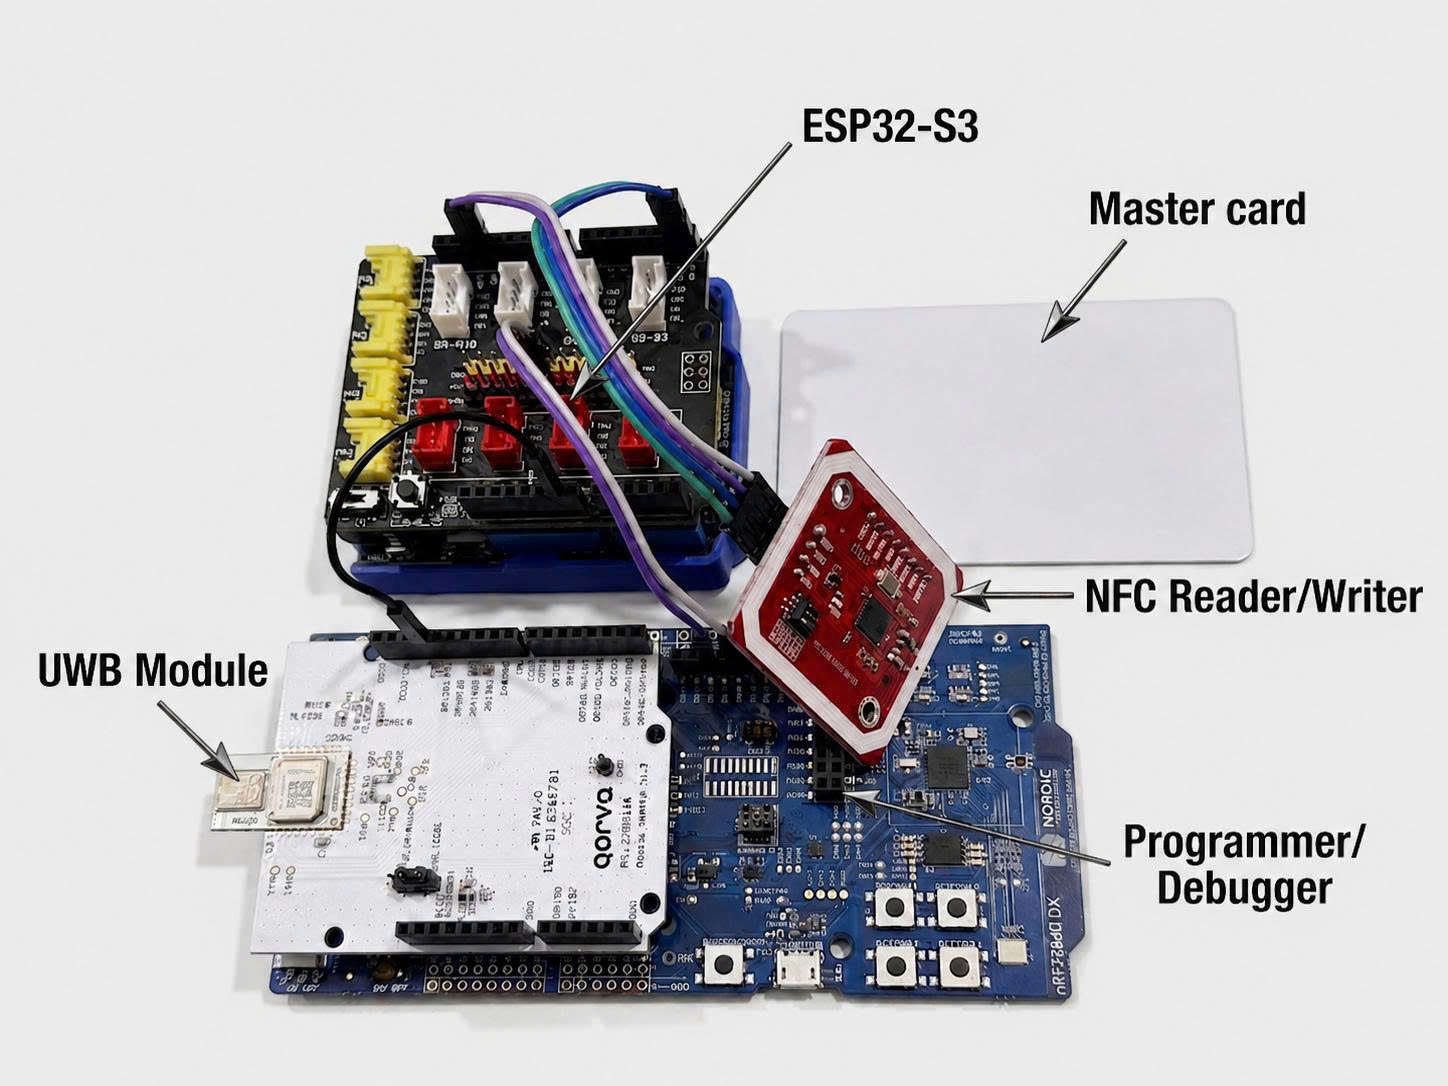
\includegraphics[width=0.8\textwidth]{image/section5/hardware.jpg} 
    \caption[Sơ đồ ghép nối hệ thống UWB đa mỏ neo]{Sơ đồ ghép nối hệ thống UWB đa mỏ neo: ESP32-S3 (trung tâm), ba mỏ neo DWM3001CDK, cầu nối PC và điện thoại Controller. \textit{(Sinh viên lưu ý cập nhật hình minh họa cho đúng cấu trúc liên kết mới.)}}
    \label{fig:uwb_hardware_arch}
\end{figure}


Sự kết hợp giữa ESP32-S3 (chuyên xử lý ứng dụng và hợp nhất dữ liệu) với ba mỏ neo DW3000 (chuyên xử lý tín hiệu UWB) và cầu nối PC (chuyên thu thập/đóng gói dữ liệu) tạo ra một hệ thống nhúng có độ tin cậy cao, mang đậm tính thực tiễn và tuân thủ chặt chẽ các thiết kế tham chiếu (Reference Design) của ngành công nghiệp ô tô hiện đại.

\begin{figure}[H]
    \centering
    \begin{minipage}{0.48\textwidth}
        \centering
        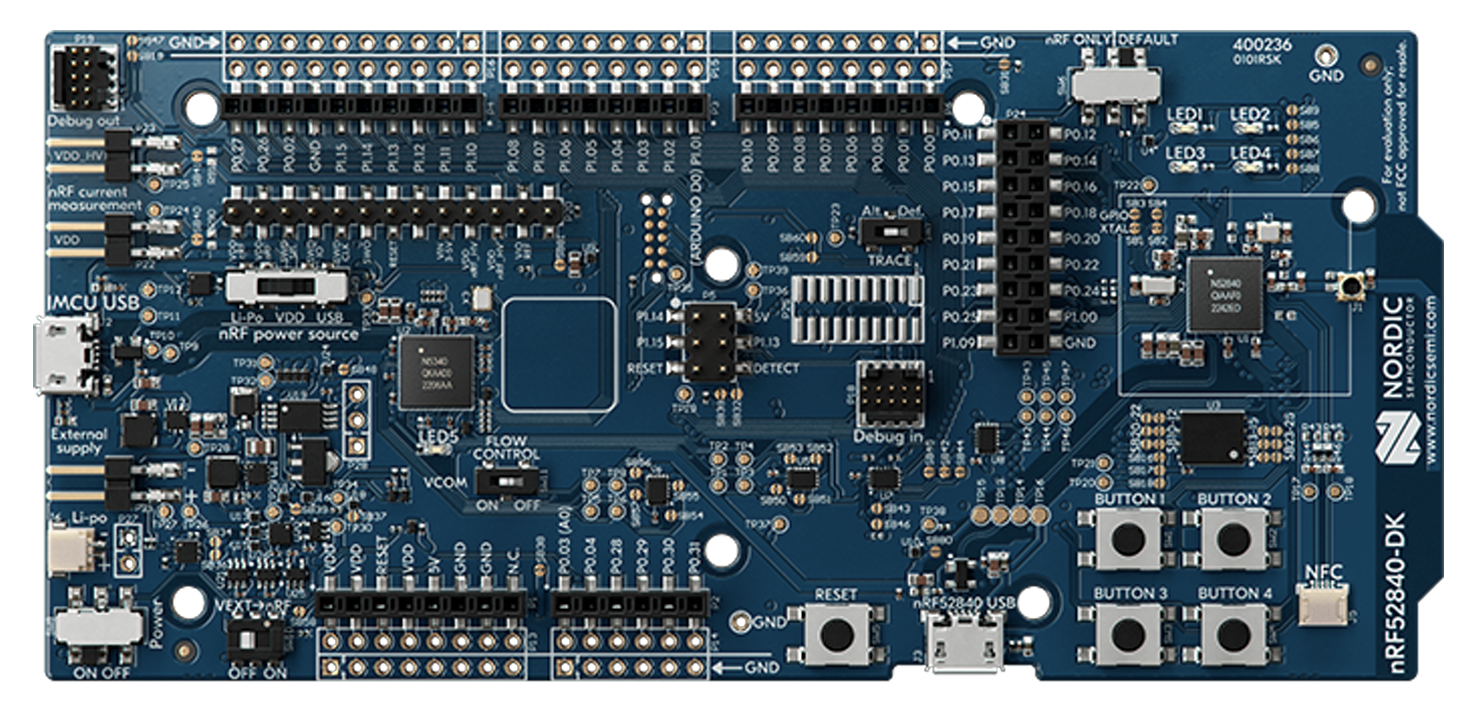
\includegraphics[width=\linewidth]{image/section5/nRF52840_DK.png}
        \caption[Mạch trung gian nRF52840]{Mạch trung gian nRF52840 (\textbf{Nguồn:} \href{https://docs.edgeimpulse.com/hardware/boards/nordic-semi-nrf52840-dk}{Nordic Semi nRF52840 DK})}
        \label{fig:hardware}
    \end{minipage}
    \hfill
    \begin{minipage}{0.48\textwidth}
        \centering
        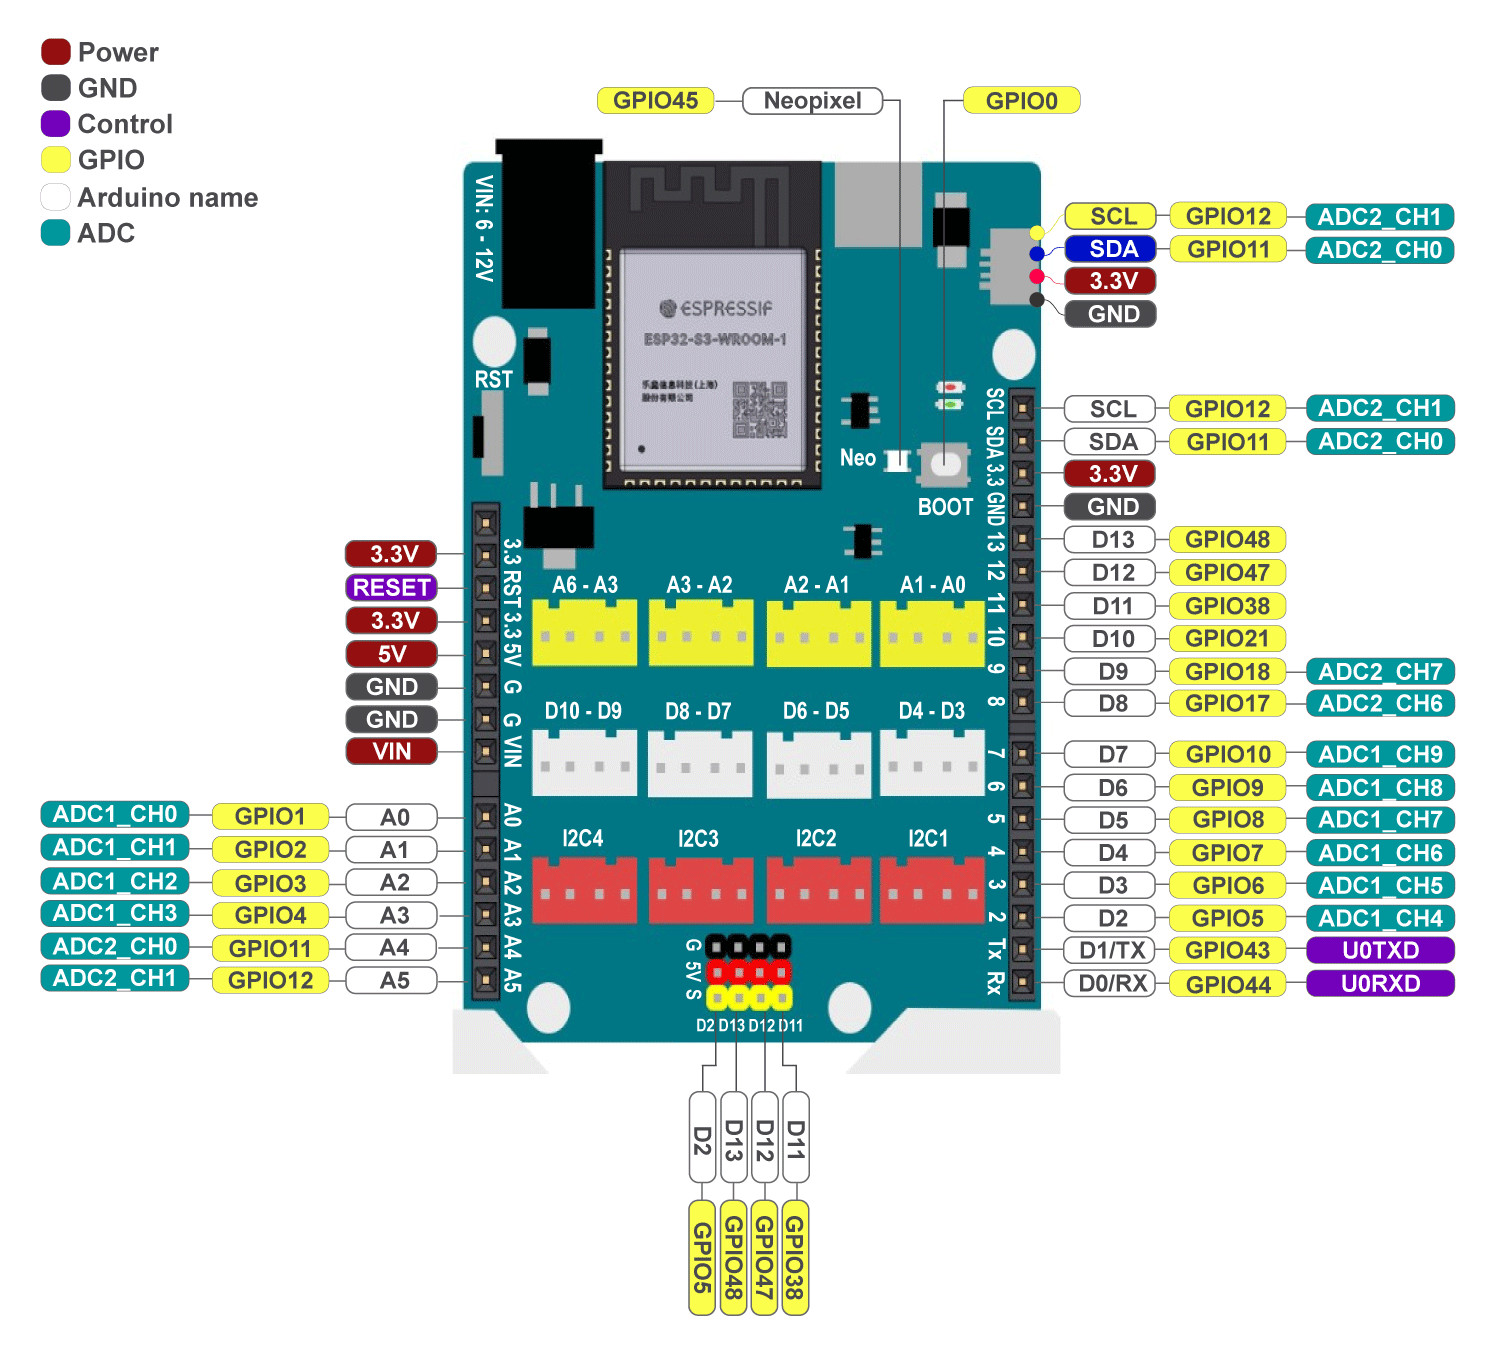
\includegraphics[width=\linewidth]{image/section5/yolouno_spec.jpg}
        \caption[Sơ đồ chân Yolo Uno ESP32-S3]{Sơ đồ chân Yolo Uno ESP32-S3 (\textbf{Nguồn:} \href{https://docs.ohstem.vn/en/latest/yolo_uno/yolo_uno_khoi_lenh/gioi_thieu_yolo_uno.html}{OhStem - Yolo UNO doc})}
        \label{fig:spec_yolouno}
    \end{minipage}
\end{figure}

\begin{figure}[H]
    \centering
    \begin{minipage}{0.38\textwidth}
        \centering
        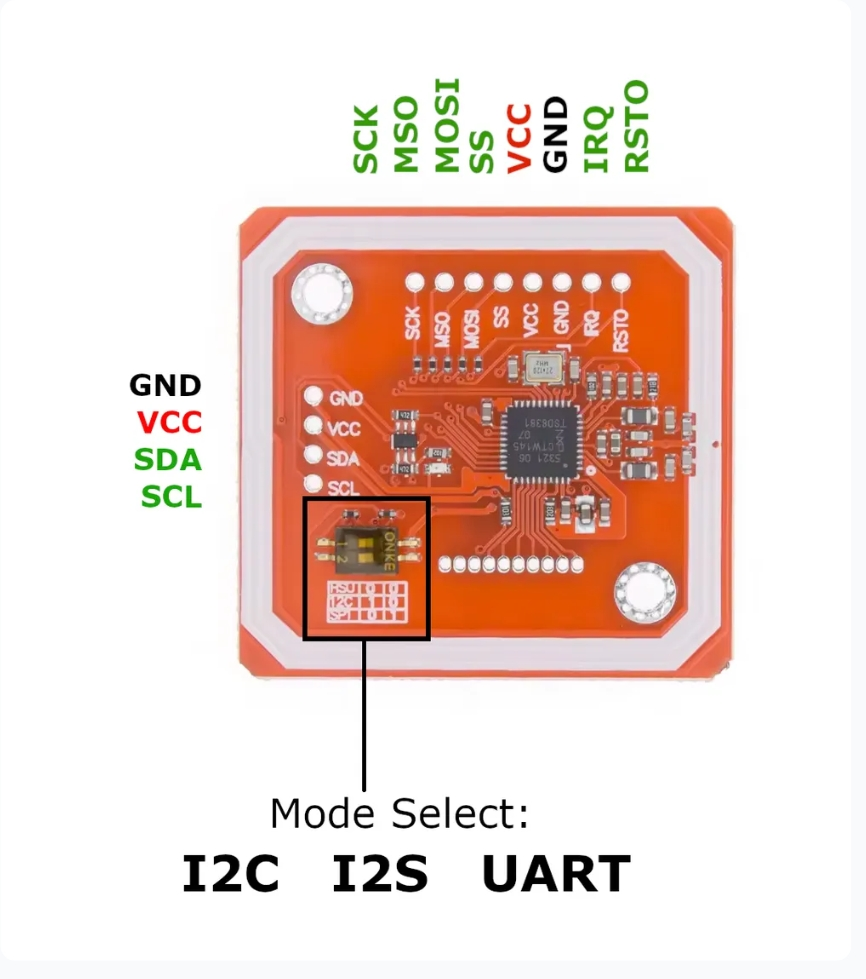
\includegraphics[width=\linewidth]{image/section5/spec_pn532.jpeg}
        \caption[Module NFC PN532]{Module NFC PN532 (\textbf{Nguồn:} \href{https://www.espboards.dev/sensors/pn532/}{ESPBoards - PN532 NFC Module Pinout})}
        \label{fig:spec_pn532}
    \end{minipage}
    \hfill
    \begin{minipage}{0.38\textwidth}
        \centering
        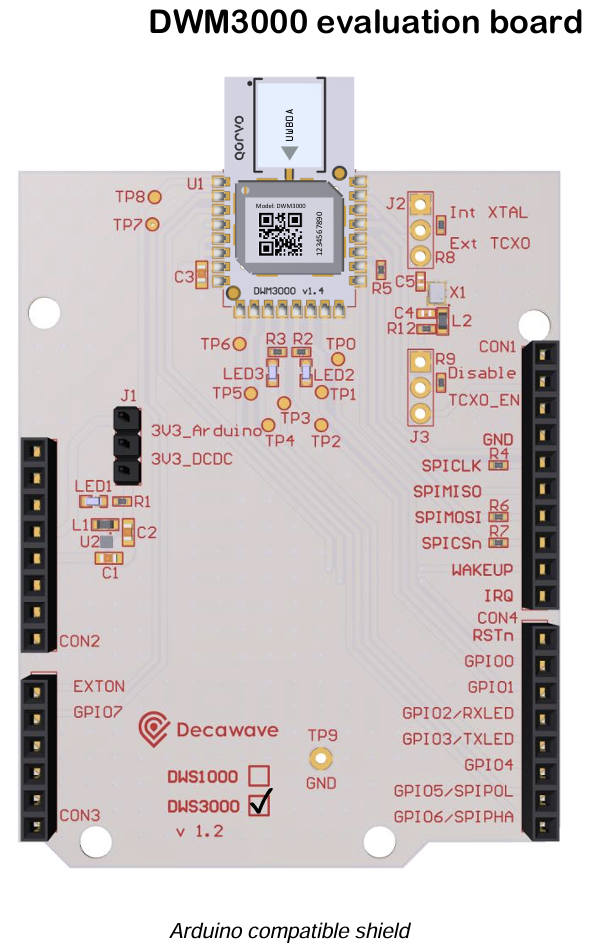
\includegraphics[width=\linewidth]{image/section5/DWM3000EVB.png} % Cập nhật tên file ảnh DWM3000EVB nếu cần
        \caption[Module UWB DWM3000EVB]{Module UWB DWM3000EVB (\textbf{Nguồn:} \href{https://www.digikey.tw/en/products/detail/qorvo/DWM3000EVB/24367408}{DWM3000EVB Qorvo - DigiKey})}
        \label{fig:spec_dwm3000}
    \end{minipage}
    \hfill
    \begin{minipage}{0.38\textwidth}
        \centering
        \includegraphics[width=\linewidth]{image/section5/DWM3001CDK.jpg} % Cập nhật tên file ảnh mỏ neo UWB nếu cần
        \caption[Mỏ neo UWB DWM3001CDK (vi mạch DW3000)]{Mỏ neo UWB DWM3001CDK (vi mạch Qorvo DW3000) (\textbf{Nguồn:} \href{https://www.qorvo.com/products/p/DWM3001CDK}{DWM3001CDK Qorvo})}
        \label{fig:spec_dwm3001cdk}
    \end{minipage}
\end{figure}








%------------------------------------------------------------------------------------






\subsection{Hiện thực phần mềm}

Kiến trúc phần mềm trên ESP32 được xây dựng trên nền tảng hệ điều hành thời gian thực FreeRTOS, cho phép các tác vụ (NFC, BLE, UWB) hoạt động đa luồng (Multi-tasking) một cách mượt mà.

\subsection{Máy trạng thái hữu hạn xuyên tầng (Cross-layer FSM)}

Cốt lõi điều khiển của ESP32 là Máy trạng thái hữu hạn (FSM) quản lý toàn bộ vòng đời truy cập. Lớp \texttt{FSMIntegration} đóng vai trò Adapter, nhận sự kiện từ các module phần cứng và điều hướng FSM.

\begin{itemize}
    \item \textbf{Khởi tạo (INIT \& IDLE):} Hệ thống duy trì quảng bá BLE và chờ quét thẻ NFC.
    \item \textbf{Cấp quyền (PROVISIONING - Phase A):} Điều khiển luồng APDU với điện thoại qua module PN532. Lưu trữ định danh điện thoại vào NVS.
    \item \textbf{Xác thực (AUTH - Phase B):} Quản lý tiến trình bắt tay mật mã (ECDH, HKDF) qua kết nối BLE. Khi hoàn tất, hệ thống đạt trạng thái \texttt{AUTH\_SECURE\_CHANNEL\_READY}.
    \item \textbf{Đo khoảng cách và Mở khóa (RANGING \& UNLOCK - Phase C \& D):} Khi nhận OOB Payload qua BLE, FSM cho phép luồng UWB Ranging hoạt động. Trạng thái \texttt{UNLOCKING\_EXECUTE} chỉ được kích hoạt khi cả kênh BLE và dữ liệu UWB đều hợp lệ.
\end{itemize}

\subsection{Xử lý NFC và Provisioning (Phase A)}
Module \texttt{nfc\_session.cpp} (chạy trên \texttt{NFCTask}) chịu trách nhiệm thiết lập kênh tin cậy ban đầu (Trust Establishment). Để khắc phục hiện tượng nhiễu tín hiệu RF, hệ thống áp dụng kỹ thuật \textit{Adaptive Polling} (chống rung tín hiệu): yêu cầu xác nhận sự hiện diện ổn định của thẻ qua nhiều chu kỳ đọc liên tiếp (\texttt{stableReads}) trước khi thiết lập kết nối APDU.

\noindent\begin{minipage}{\linewidth}
\begin{lstlisting}[language=C++, caption={Adaptive Polling logic cho NFC}]
bool waitForCard(uint32_t timeoutMs = 15000, uint8_t stableReads = 2) {
    while (true) {
        // Debounce logic: Request for successive stability detection
        if (nfc->inListPassiveTarget()) {
            if (++stableCount >= stableReads) return true;
        } else {
            stableCount = 0; // Reset if signal is lost.
        }
    }
}
\end{lstlisting}
\end{minipage}

Quy trình APDU bao gồm: Lựa chọn Applet (\texttt{SELECT AID}), trao đổi thông tin định danh, xác thực chữ ký số bằng thuật toán ECDSA. Nếu thành công, thiết bị sẽ được lưu vào danh sách truy cập (NVS).

\subsection{Giao thức xác thực BLE (Phase B)}
Giai đoạn này thiết lập kênh truyền an toàn không dây. Để tránh gây nghẽn (timeout) cho kết nối BLE do các phép toán mật mã đường cong Elliptic tốn nhiều tài nguyên, hệ thống tách các phép toán này vào một FreeRTOS Task độc lập (\texttt{AuthWorker}). Quy trình mật mã tuân thủ cấu trúc ECDH Ephemeral:

\noindent\begin{minipage}{\linewidth}
\begin{lstlisting}[language=C++, caption={Các bước mật mã chính trong Phase B}]
// 1. Generate Ephemeral P-256 (Forward Secrecy) key pair
mbedtls_ecp_gen_keypair(&grp, &d, &Q, rng, &ctr_drbg);

// 2. Calculating Shared Secrets (ECDH)
mbedtls_ecdh_compute_shared(&grp, &z, &Qp, &d, rng, &ctr_drbg);

// 3. Derive Session Keys using HKDF-SHA256
mbedtls_hkdf(md_info, salt, saltLen, ikm, ikmLen, info, infoLen, output, 32);
\end{lstlisting}
\end{minipage}

Hàm HKDF sẽ tách Shared Secret thành hai khóa độc lập: Session Encryption Key (để mã hóa AES-GCM) và Session MAC Key (để xác thực HMAC).

\subsection{Đo khoảng cách đa mỏ neo và Định vị Trilateration (Phase C)}
Đây là trọng tâm vật lý của hệ thống. Sau khi xác thực BLE (Phase B), điện thoại gửi lệnh \texttt{RANGING\_START} qua đường hầm CCC. ESP32 (lớp \texttt{UwbBridge}) chuyển thành lệnh \texttt{CMD:START\_RANGING} gửi sang cầu nối PC, cầu nối này khởi tạo phiên DS-TWR multicast trên ba mỏ neo.

Trong mỗi vòng đo, điện thoại (Controller) trao đổi xung với cả ba mỏ neo (Responder) theo giao thức \textbf{Symmetrical Double-Sided Two-Way Ranging (DS-TWR)}. Cầu nối PC thu thập ba khoảng cách $d_0, d_1, d_2$, kiểm tra tính tươi (freshness) và phạm vi hợp lệ $[0.1,\,30]$ m, rồi đóng gói thành một dòng văn bản gửi sang ESP32 qua USB-CDC:

\noindent\begin{minipage}{\linewidth}
\begin{lstlisting}[language=C++, caption={Khung dữ liệu RANGE và hàm phân tích trên ESP32}]
// Frame received from PC bridge over USB-CDC:
//   RANGE:d0=1.82,d1=0.97,d2=3.14,valid=1
bool UwbBridge::parseRange(const char* line, RangingFrame& frame) {
    double d0, d1, d2; int valid;
    if (sscanf(line, "RANGE:d0=%lf,d1=%lf,d2=%lf,valid=%d",
               &d0, &d1, &d2, &valid) != 4) return false;
    frame.d[0] = d0; frame.d[1] = d1; frame.d[2] = d2;
    frame.valid_mask = valid ? 0x07 : 0x00;   // 0b111 when all three are valid
    frame.t_ms = millis();
    return true;
}
\end{lstlisting}
\end{minipage}

Cờ \texttt{valid} chỉ được bật khi \textbf{cả ba} khoảng cách đều tươi và nằm trong phạm vi hợp lệ. Khi đủ điều kiện, ESP32 tiến hành định vị hai bước: \texttt{Trilateration::solve} trả về tọa độ $(x, y)$ kèm chất lượng lời giải RMS, sau đó \texttt{Ekf::update} hợp nhất phép đo vào quỹ đạo:

\noindent\begin{minipage}{\linewidth}
\begin{lstlisting}[language=C++, caption={Định vị Trilateration và cập nhật EKF}]
// 1. Trilateration: 3 khoang cach -> toa do (x, y) + chat luong RMS
Trilateration::Result fix = Trilateration::solve(frame.d, frame.valid_mask);

// 2. EKF: cap nhat vi tri, uoc luong van toc (x, y, vx, vy)
if (fix.valid) {
    double sigma = clamp(fix.rms, 0.05, 1.0);   // nhieu do ~ chat luong loi giai
    ekf.update(fix.x, fix.y, frame.t_ms, sigma);
}
ekf.predictTo(millis());   // du bao bu khi mat khung du lieu
\end{lstlisting}
\end{minipage}

Bộ lọc Kalman hai chiều chạy ở nhịp cố định 10 Hz, độc lập với nhịp nhận khung dữ liệu, và tự động dự báo bù khi một vài khung bị mất (tối đa 2 giây).

\subsection{Quyết định truy cập theo vùng hình học (Phase D)}

Sau khi bộ lọc Kalman hai chiều cung cấp trạng thái mượt $(x, y, v_x, v_y)$ ở nhịp 10 Hz, hệ thống thực hiện \textbf{phân vùng không gian} (Geofencing) và ra quyết định truy cập thông qua một \textbf{máy trạng thái truy cập} gồm ba trạng thái. Đây là tầng lõi tất định (deterministic) của hệ thống, hoạt động độc lập với tầng học sâu, đảm bảo tính an toàn cơ học (fail-safe) ngay cả khi tầng AI chưa sẵn sàng.

\subsubsection{Phân vùng không gian (Geofencing)}

Module \texttt{Geofence} ánh xạ tọa độ đã lọc $(x, y)$ vào bốn vùng ảo trong hệ quy chiếu gắn với xe (gốc tọa độ tại tâm xe, $+x$ hướng sang phải, $+y$ hướng về phía trước):

\begin{itemize}
    \item \textbf{DRIVER\_SEAT:} vùng ghế lái, tâm $(-0.35,\,0)$ bán kính $0.45$ m --- đại diện vị trí người dùng ngồi vào xe.
    \item \textbf{DRIVER\_DOOR:} vùng cửa tài xế, tâm $(-0.95,\,0)$ bán kính $2.0$ m (trùng với mỏ neo $A_2$ --- cột B bên trái).
    \item \textbf{WELCOME:} vùng chào đón, bán kính $4.0$ m tính từ tâm xe.
    \item \textbf{OUTSIDE:} bên ngoài vùng chào đón.
\end{itemize}

Bộ lọc \texttt{Hysteresis} chỉ chấp nhận vùng ổn định (đồng nhất trong 3 chu kỳ liên tiếp) nhằm triệt tiêu hiện tượng chuyển vùng liên tục tại biên giới (boundary chatter).

\subsubsection{Máy trạng thái truy cập (Access State Machine)}

Module \texttt{AccessController} duy trì ba trạng thái hoạt động:

\begin{itemize}
    \item \textbf{LOCKED:} cửa khóa, chưa cấp quyền khởi động.
    \item \textbf{DOOR\_UNLOCKED:} cửa đã mở, người dùng chưa ngồi vào ghế lái.
    \item \textbf{OCCUPIED:} người dùng đã ngồi vào ghế lái --- cửa khóa lại và cấp quyền khởi động động cơ.
\end{itemize}

Các chuyển trạng thái được điều khiển bởi các cổng tất định:

\begin{enumerate}
    \item \textbf{Mở khóa} (\texttt{LOCKED $\rightarrow$ DOOR\_UNLOCKED}): chỉ khi người dùng ở vùng cửa (\texttt{DRIVER\_DOOR}/\texttt{DRIVER\_SEAT}), \textbf{giảm tốc gần như dừng hẳn} (tốc độ $< 0.4$ m/s) trong 3 chu kỳ liên tiếp, đồng thời không có chuyển động rời xa (cổng vận tốc hướng tâm).
    \item \textbf{Định cư ghế lái} (\texttt{DOOR\_UNLOCKED $\rightarrow$ OCCUPIED}): khi người dùng đứng yên trong vùng \texttt{DRIVER\_SEAT} liên tục 3 giây. Lúc này hệ thống khóa cửa và cấp quyền khởi động (chân \texttt{GPIO27}).
    \item \textbf{Rời đi} (\texttt{OCCUPIED $\rightarrow$ LOCKED}): khi người dùng ra khỏi vùng chào đón (\texttt{OUTSIDE}) và có vận tốc hướng ra xa trong 3 chu kỳ liên tiếp. Hệ thống thu hồi quyền khởi động và khóa cửa.
    \item \textbf{Hủy bỏ} (\texttt{DOOR\_UNLOCKED $\rightarrow$ LOCKED}): người dùng bỏ đi mà không ngồi vào ghế --- hệ thống khóa cửa trở lại.
\end{enumerate}

Trong đó, \textbf{cổng giảm tốc} (deceleration gate) là bổ sung quan trọng: yêu cầu người dùng phải giảm tốc gần như dừng hẳn ở gần cửa mới được mở khóa, nhờ đó loại bỏ triệt để các trường hợp người dùng chỉ \textit{đi ngang qua} cửa (tangential pass) mà không có ý định vào xe --- điều mà một ngưỡng vận tốc hướng tâm đơn thuần không thể phân biệt được.

\noindent\begin{minipage}{\linewidth}
\begin{lstlisting}[language=C++, caption={Máy trạng thái truy cập (AccessController) rút gọn}]
void AccessController::handlePosition(double x, double y,
                                      double vx, double vy) {
  double vr = radialSpeed(x, y, vx, vy);          // >0 roi xa, <0 tien lai
  Zone  z  = zone_hyst.update(x, y, 3);           // vung on dinh (debounce 3)
  bool movingAway = (vr > 0.10);
  double speed = hypot(vx, vy);

  switch (state_) {
    case LOCKED:
      if (z == OUTSIDE || movingAway) { hits = 0; return; }
      if ((z == DRIVER_DOOR || z == DRIVER_SEAT) && speed < 0.4) {
        if (++hits >= 3) { fireUnlock(); state_ = DOOR_UNLOCKED; hits = 0; }
      } else hits = 0;
      break;
    case DOOR_UNLOCKED:
      if (z == DRIVER_SEAT && speed < 0.4) {       // ngoi yen ghe lai 3s
        if (settledFor(3s)) { lockDoor(); setIgnition(true); state_ = OCCUPIED; }
      }
      if (z == OUTSIDE && movingAway) { lockDoor(); state_ = LOCKED; }
      break;
    case OCCUPIED:
      if (z == OUTSIDE && movingAway) {            // roi di
        if (++leaveHits >= 3) { setIgnition(false); lockDoor(); state_ = LOCKED; }
      } else leaveHits = 0;
      break;
  }
}
\end{lstlisting}
\end{minipage}

\subsubsection{Kích hoạt cơ cấu chấp hành}

Kết quả ra quyết định được phản ánh qua hai kênh tín hiệu:

\begin{itemize}
    \item \textbf{Chân \texttt{GPIO26}}: điều khiển rơ-le khóa/mở cửa --- mức \texttt{LOW} tương ứng trạng thái khóa, xung \texttt{HIGH} trong 500 ms tương ứng lệnh mở cửa.
    \item \textbf{Chân \texttt{GPIO27}}: tín hiệu cấp quyền khởi động động cơ --- mức \texttt{HIGH} khi ở trạng thái \texttt{OCCUPIED}.
\end{itemize}

Toàn bộ quy trình chuyển trạng thái được ghi nhận qua các thẻ log \texttt{[ZONE]}, \texttt{[STATE]} và \texttt{[IGNITION]} phục vụ giám sát và kiểm thử. Logic tất định này tạo ra trải nghiệm \textit{Passive Keyless Entry} mượt mà: mở cửa khi người dùng tiến lại gần và dừng lại, khóa cửa và cấp quyền khởi động khi người dùng đã định cư ghế lái, rồi khóa xe và thu hồi quyền khi người dùng rời đi.






%------------------------------------------------------------------------------------






\section{Triển khai phần ứng dụng di động}

Mặc dù Flutter được sử dụng làm framework phát triển chính, nhưng đối với một hệ thống yêu cầu bảo mật phần cứng nghiêm ngặt như Smart Car Access (chuẩn CCC), ứng dụng được thiết kế theo kiến trúc phân tầng sâu. Flutter chỉ đóng vai trò là Lớp Giao diện (Presentation) và Điều phối logic (Domain), trong khi toàn bộ các tác vụ mật mã và điều khiển phần cứng vô tuyến được chuyển giao (delegate) xuống tầng Native Android (Kotlin).

\subsection{Tích hợp Native Android}
Ứng dụng thiết lập một hệ thống \texttt{MethodChannel} và \texttt{EventChannel} để ánh xạ trực tiếp các lệnh từ Dart xuống API hệ thống của Android:

\begin{itemize}
    \item \textbf{Kênh \texttt{smartcar/keystore}:} Chịu trách nhiệm quản lý định danh. Native Kotlin (\texttt{KeystoreBridge.kt}) trực tiếp sinh cặp khóa ECDSA P-256 và bảo vệ Private Key vĩnh viễn trong vùng an toàn (Hardware-backed) của Android Keystore. Các thao tác ký điện tử ở Phase A được thực hiện tại đây để khóa bí mật không bao giờ lọt lên tầng Flutter.
    \item \textbf{Kênh \texttt{smartcar/mastercard} \& \texttt{smartcar/nfc\_reader}:} Quản lý phiên cấp quyền (Provisioning Session). Module \texttt{MasterCardSession} nhận dữ liệu xác thực từ Flutter và giữ phiên làm việc tạm thời trong RAM để cấp phép cho tiến trình mô phỏng thẻ HCE hoạt động.
    \item \textbf{Kênh \texttt{smartcar/uwb}:} Lớp \texttt{UwbRangingBridge.kt} gọi trực tiếp API \texttt{androidx.core.uwb} của hệ điều hành, cấu hình các tham số Ranging chuẩn FiRa (Channel, Preamble Index, MAC) và sử dụng Coroutine để duy trì vòng lặp đo khoảng cách liên tục, đẩy dữ liệu tọa độ về Flutter qua luồng sự kiện.
\end{itemize}

\subsection{Cấp quyền vật lý qua Thẻ chủ (Phase A - Master Card \& HCE)}
Luồng cấp quyền (Provisioning) được chia làm hai bước tách biệt nhằm tối đa hóa bảo mật:
\begin{enumerate}
    \item \textbf{Xác nhận chủ sở hữu (Flutter):} Người dùng sử dụng Flutter App (\texttt{Master CardProvisioningService}) để quét thẻ vật lý Master Card (chứa NDEF Payload gồm \texttt{vid} và \texttt{msk}). Dữ liệu này được đẩy xuống tầng Native thông qua MethodChannel để mở khóa phiên làm việc.
    \item \textbf{Giao tiếp APDU (Native HCE):} Ngay sau đó, dịch vụ \texttt{Provisioning HostApduService} (chạy ngầm dưới nền hệ điều hành) tiếp quản. Dịch vụ này mô phỏng thẻ thông minh (AID \texttt{F00102030405}), thực hiện cơ chế xác thực SPAKE2+ từ Master Card, trao đổi khóa và ký Challenge bằng Android Keystore, hoàn toàn độc lập với vòng đời của giao diện Flutter.
\end{enumerate}

\subsection{Cơ chế chạy ngầm và Bàn giao phần cứng}
Để hiện thực hóa tính năng "Mở khóa thụ động" (Passive Keyless Entry) mà không cần người dùng mở màn hình điện thoại, ứng dụng áp dụng kiến trúc \textit{Dual-Isolate}:

\begin{itemize}
    \item \textbf{Background Isolate:} Chạy liên tục dưới dạng Android Foreground Service (\texttt{Pke BackgroundService.dart}). Luồng này lắng nghe sóng BLE, tự động kết nối và thực hiện toàn bộ luồng mật mã ECDH (Phase B) một cách âm thầm.
    \item \textbf{Foreground Isolate:} Đảm nhiệm cấu hình chip UWB. Do các chính sách bảo mật hệ thống của Android, phần cứng UWB chỉ cho phép khởi tạo khi ứng dụng đang ở trên màn hình (Foreground).
\end{itemize}

Để giải quyết bài toán chuyển tiếp giữa hai luồng độc lập mà không làm đứt kết nối BLE (gây trễ do phải quét lại), đề tài áp dụng cơ chế \textbf{Connection Hold \& Handoff}. Luồng Background sau khi xác thực BLE thành công sẽ \textbf{không gửi lệnh ngắt kết nối}, mà phát tín hiệu đánh thức luồng Foreground. Luồng Foreground lập tức tiếp quản kết nối BLE thông qua địa chỉ MAC đã biết, vá địa chỉ UWB cục bộ vào OOB Payload, gửi cho ESP32 và bật chip UWB. Thiết kế này giúp giảm thời gian chuyển tiếp từ Phase B sang Phase C xuống dưới 400ms.

\subsection{Dữ liệu và Hệ thống cảnh báo an ninh}
Ứng dụng sử dụng Firebase Firestore (\texttt{CarService.dart}) để đồng bộ hóa trạng thái xe và khóa số theo thời gian thực. Toàn bộ các thao tác ghi dữ liệu đều được ràng buộc bảo mật với \texttt{ownerId} của Firebase Auth.

Bên cạnh đó, ứng dụng tích hợp dịch vụ thu thập tọa độ \texttt{GpsService}. Dữ liệu GPS không chỉ dùng để hiển thị mà được đóng gói thành một cấu trúc nhị phân 32-byte, mã hóa tính toàn vẹn bằng HMAC-SHA256 và gửi qua BLE. Hệ thống AI (\texttt{AnomalyDetectionService}) sẽ tổng hợp các sự kiện truy cập, phân tích yếu tố thời gian/vị trí để phát cảnh báo đẩy (Push Notification) nếu phát hiện hành vi truy cập bất thường.

\subsection{Giao diện Kiểm thử Chuyên sâu (Integration Test UIs)}
Khác với các ứng dụng thông thường, giao diện hệ thống này được thiết kế đi kèm với các công cụ kiểm thử tích hợp chuyên biệt, cho phép cô lập và đánh giá từng giao thức vô tuyến trong kiến trúc Tri-Radio. Có hai màn hình kiểm thử chính:

\begin{itemize}
    \item \textbf{Giao diện Kiểm thử Phase A/B (\texttt{TestPhaseABScreen}):} 
    Chuyên dùng để kiểm tra tính toàn vẹn của Android Keystore và luồng BLE. Màn hình này mô phỏng lại các bước của dịch vụ HCE, kiểm tra sự tồn tại của khóa Identity P-256. Trong Phase B, giao diện cho phép chọn thiết bị, thực hiện luồng bắt tay ECDH và in trực tiếp các log mật mã (Shared Secret, Session Keys, Challenge) ra màn hình Console nội bộ nhằm đối chiếu với log trên ESP32.
    
    \item \textbf{Giao diện Kiểm thử UWB (\texttt{TestUwbScreen}):} 
    Được thiết kế chuyên biệt để gỡ lỗi quá trình Ranging đa mỏ neo. Màn hình cho phép các nhà phát triển kích hoạt phiên đo (Start/Stop Ranging), gửi lệnh qua đường hầm CCC, đồng thời hiển thị trực tiếp ba khoảng cách $d_0, d_1, d_2$ và trạng thái phiên từ API Native UWB (\texttt{android.ranging}) với tần số làm mới cao.
\end{itemize}

Việc tách biệt hai màn hình kiểm thử này giúp rút ngắn đáng kể thời gian gỡ lỗi phần cứng, đồng thời cung cấp công cụ trực quan để minh chứng sự hoạt động độc lập và liền mạch của các giao thức NFC, BLE và UWB trong hệ thống.






\section{Kết quả kiểm thử thực tế}

Để đảm bảo tính đúng đắn và độ ổn định của giao thức, hệ thống tích hợp các giao diện Debug chuyên dụng, cho phép cô lập và theo dõi trạng thái của từng giai đoạn, đồng thời xuất logs chi tiết từ Console.

\leavevmode
\begin{figure}[htbp]
    \centering
    \begin{minipage}{0.25\textwidth}
        \centering
        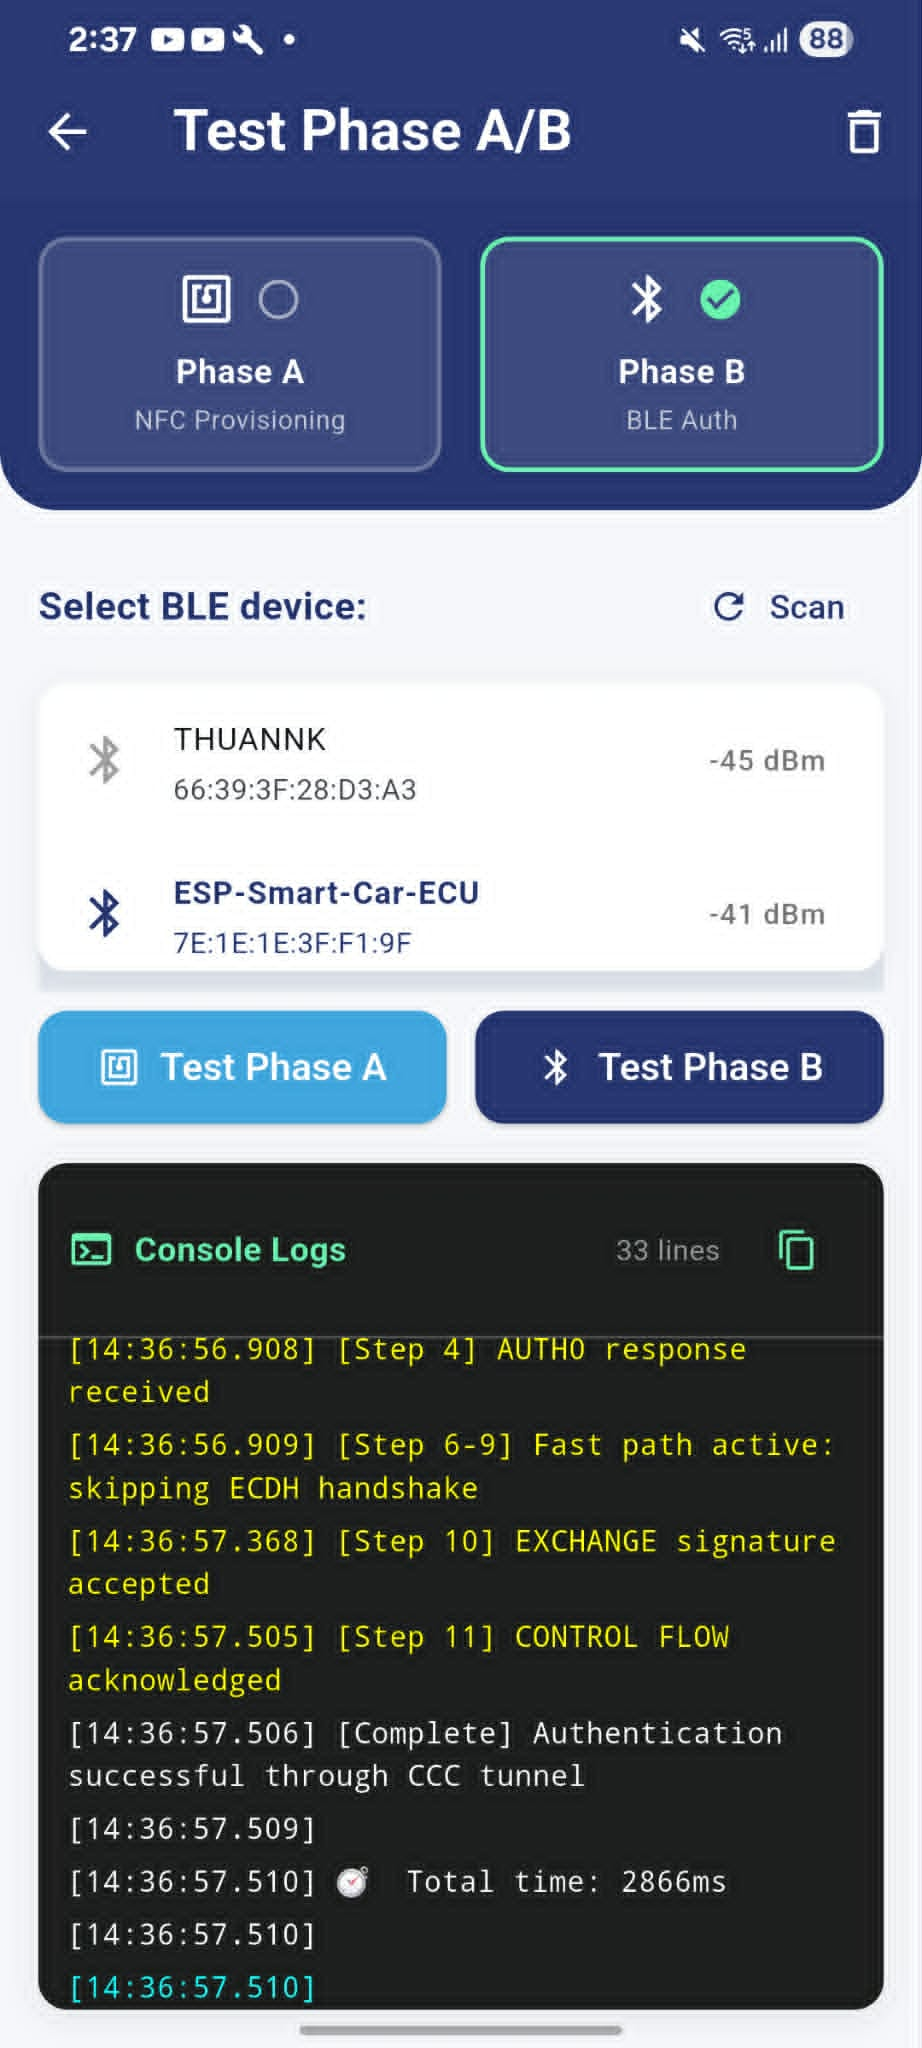
\includegraphics[width=\linewidth]{image/section5/ble_screen.jpg}
        \caption{Giao diện kiểm thử xác thực BLE (Phase B)}
        \label{fig:ble_test}
    \end{minipage}
    \hfill
    \begin{minipage}{0.25\textwidth}
        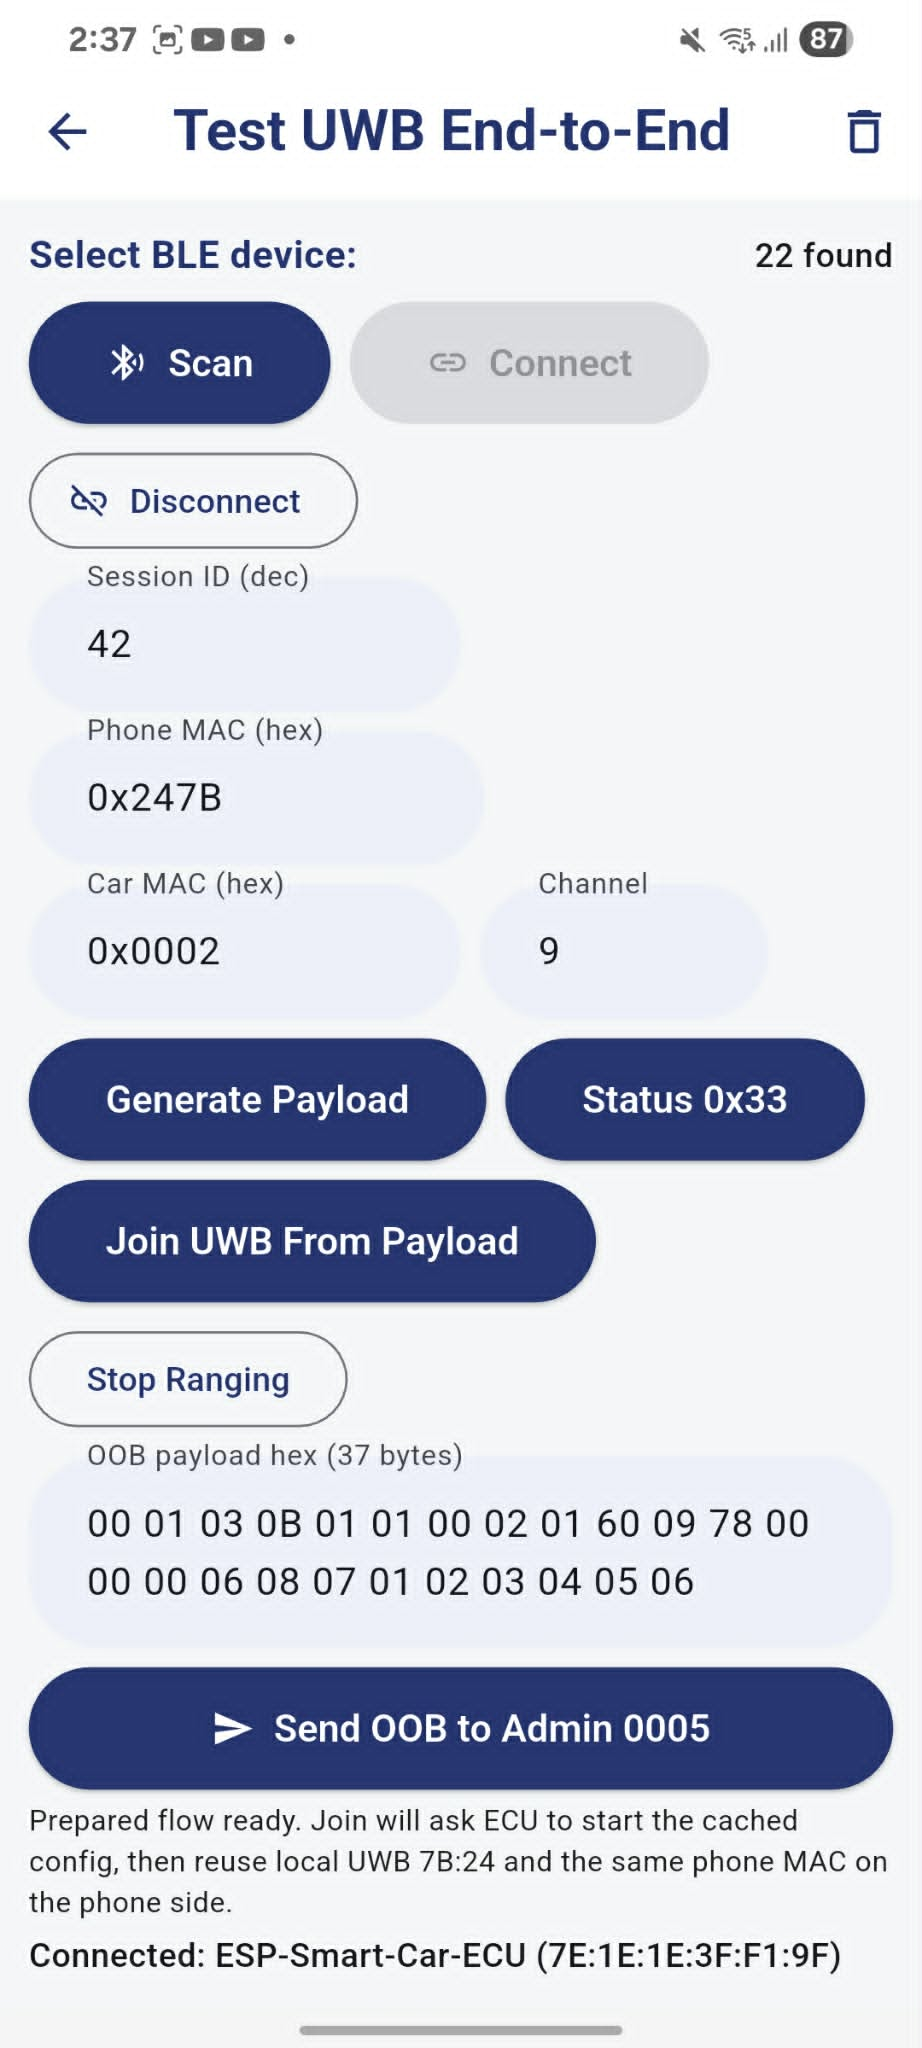
\includegraphics[width=\linewidth]{image/section5/uwb_screen_1.jpg}
        \caption{Giao diện kích hoạt UWB Ranging đa mỏ neo (Phase C) (1)}
        \label{fig:uwb_test1}
    \end{minipage}
    \hfill
    \begin{minipage}{0.25\textwidth}
        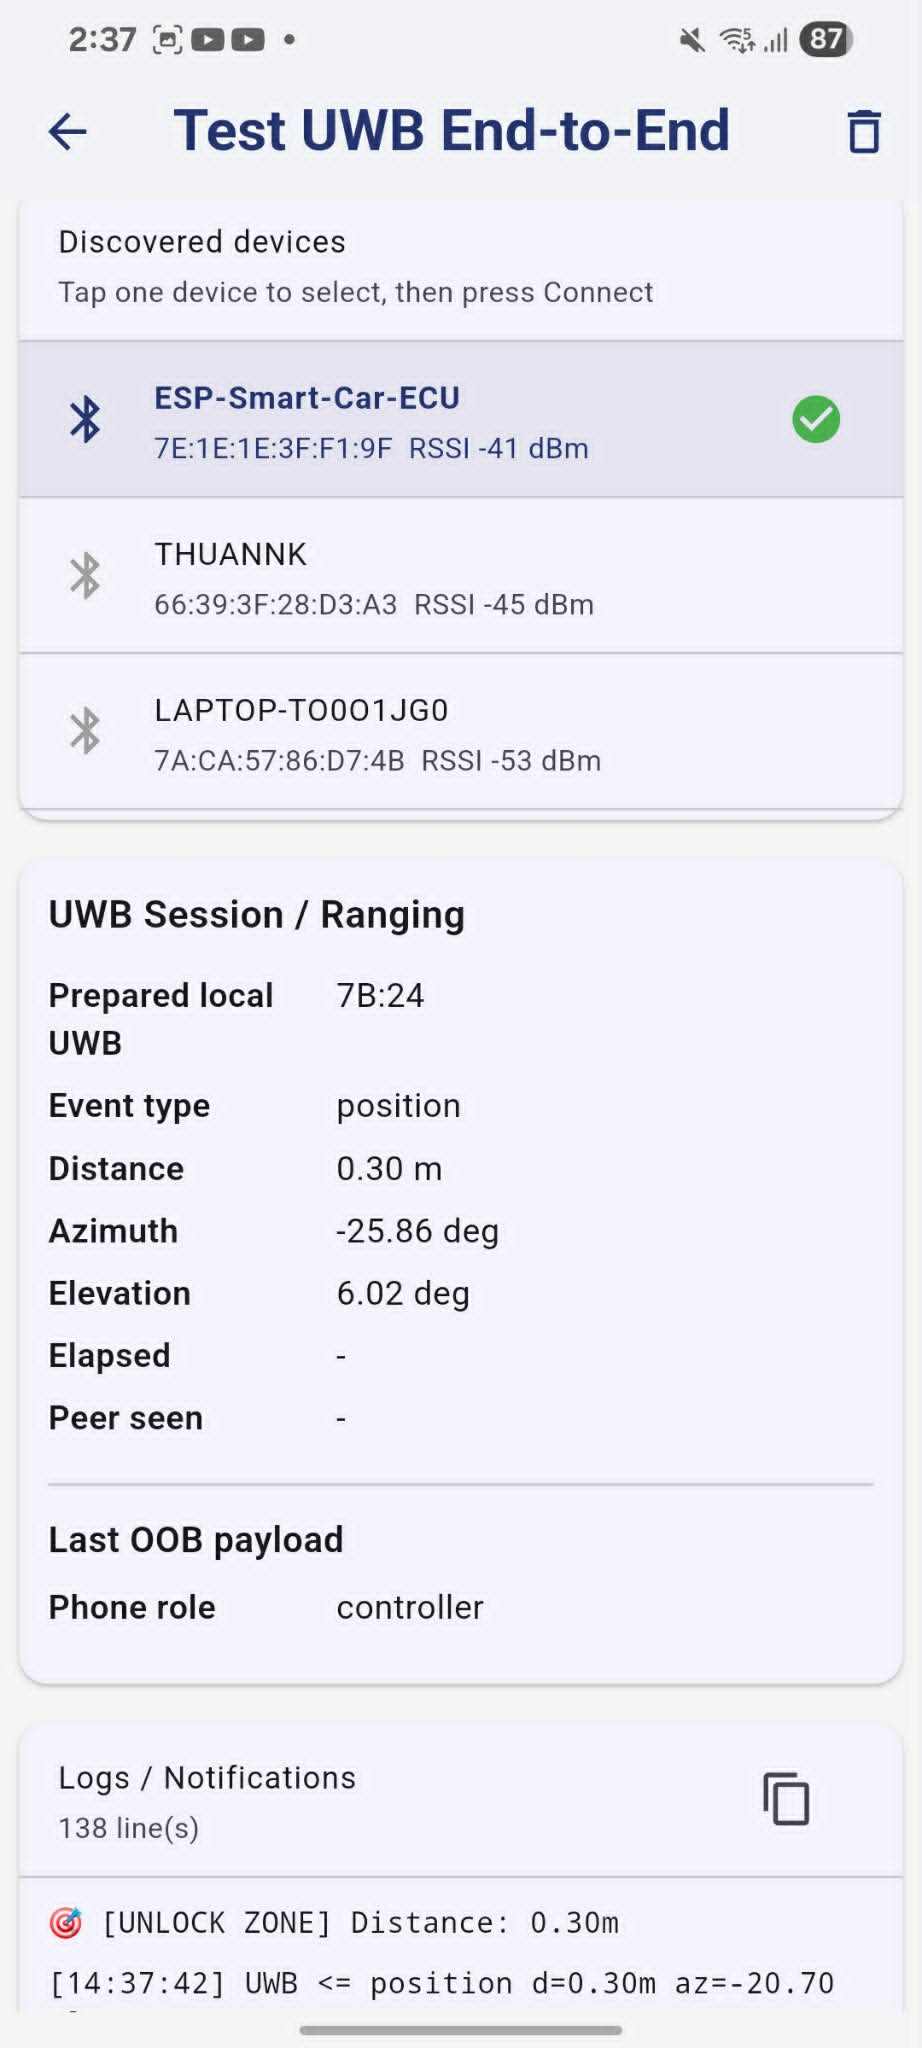
\includegraphics[width=\linewidth]{image/section5/uwb_screen_2.jpg}
        \caption{Giao diện ranging UWB Ranging (Phase C) (2)}
        \label{fig:uwb_test2}
    \end{minipage}
\end{figure}

Trong bài kiểm thử Phase B (Hình \ref{fig:ble_test}), ứng dụng tiến hành quét thiết bị BLE, thiết lập kênh an toàn và thực hiện quy trình bắt tay mật mã ECDH. Màn hình Debug hiển thị minh bạch các tham số dẫn xuất như Shared Secret và Session Keys, khẳng định kênh liên lạc đã được mã hóa an toàn.

Ngay sau khi quá trình Hand-off hoàn tất, giao diện chuyển sang bài kiểm thử Phase C (Hình \ref{fig:esp32_log}). Điện thoại thực hiện DS-TWR đồng thời với ba mỏ neo, ba khoảng cách (ví dụ: $d_0 = 1.82$m, $d_1 = 0.97$m, $d_2 = 3.14$m) được cập nhật liên tục trên màn hình, chứng minh sự đồng bộ giữa Android UWB API (\texttt{android.ranging}) và ba mỏ neo DWM3001CDK qua cầu nối PC.

\leavevmode
\begin{figure}[htbp]
	\centering
	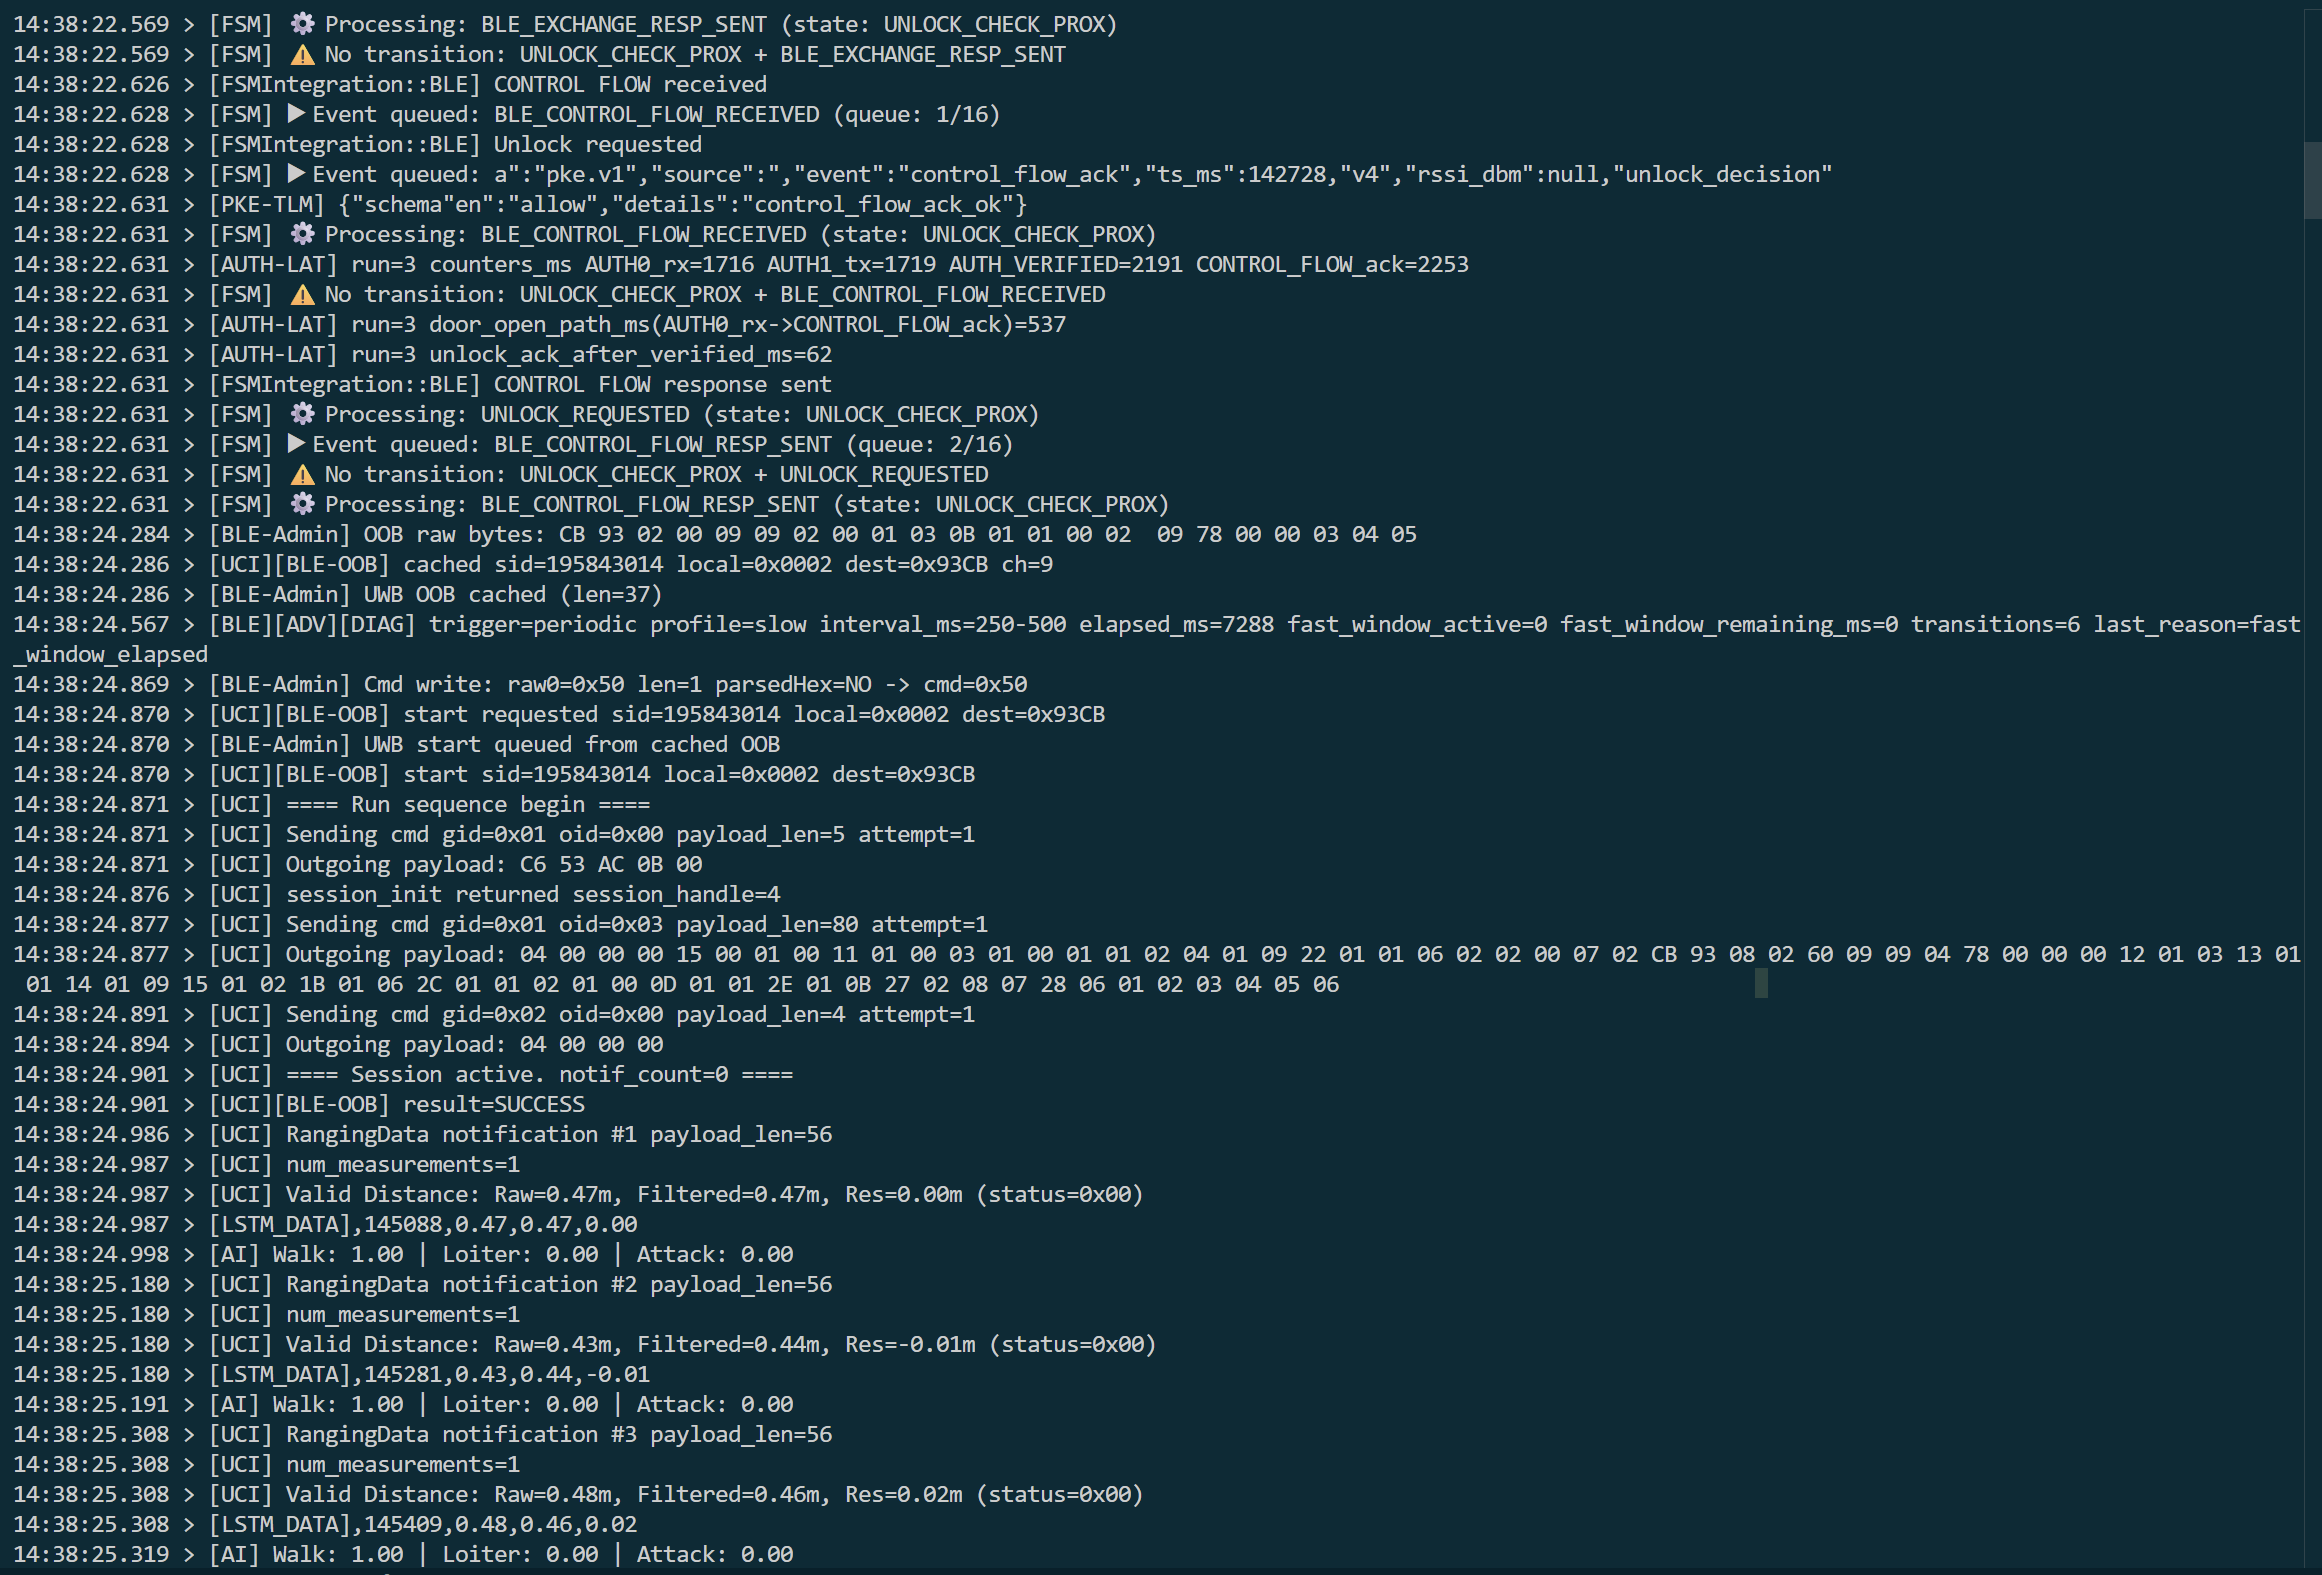
\includegraphics[width=1.0\textwidth]{image/section5/BLE TO UWB.png}
	\caption{Log xử lý xuyên tầng (BLE \& UWB) trên ESP32}
	\label{fig:esp32_log}
\end{figure}

Đối chứng từ phía vi điều khiển, log từ Serial Monitor của ESP32 (Hình \ref{fig:esp32_log}) xác nhận sự kết hợp chính xác của toàn bộ quy trình. Luồng log ghi nhận các sự kiện theo đúng thứ tự thiết kế:
\begin{enumerate}
    \item \textbf{Xác thực BLE:} Sinh khóa ephemeral, nhận Handshake, xác minh chữ ký điện thoại, tính toán ECDH và dùng HKDF sinh ra Session Keys.
    \item \textbf{Kích hoạt phiên Ranging:} Tiếp nhận lệnh \texttt{RANGING\_START} qua đường hầm CCC, ESP32 phát lệnh \texttt{CMD:START\_RANGING} sang cầu nối PC để khởi động ba mỏ neo.
    \item \textbf{Xử lý định vị thời gian thực (Trilateration + Kalman Filtering):} Ba khoảng cách thô $d_0, d_1, d_2$ từ cầu nối PC được đưa qua thuật toán Trilateration để giải tọa độ $(x, y)$, sau đó cập nhật bộ lọc Kalman hai chiều. Log hệ thống ghi nhận quá trình làm mượt quỹ đạo, triệt tiêu các xung nhiễu vật lý và ước lượng vận tốc $(v_x, v_y)$. Đây là bước tiền xử lý quan trọng để tạo ra bộ dữ liệu đầu vào ổn định cho tầng quyết định truy cập.
    \item \textbf{Suy luận ý định hành vi (On-device Inference, đang hiện thực):} Sau khi tích lũy đủ cửa sổ thời gian 25 frames, module \texttt{TrajInference} (Conv1D/TFLM) sẽ thực hiện dự báo ý định. Log Console dự kiến hiển thị các xác suất phân loại $p_{\text{approach}}$, $p_{\text{seated}}$, $p_{\text{leave}}$ và $p_{\text{passing}}$ qua thẻ log \texttt{[INTENT]}. Kết quả kỳ vọng là mô hình phản hồi $p_{\text{approach}} \ge 0.80$ khi người dùng tiến lại gần và giảm tốc.
    \item \textbf{Quyết định truy cập thông minh (AI-driven Decision, đang hiện thực):} Thay vì chỉ dựa vào ngưỡng khoảng cách vô hướng, lệnh mở GPIO rơ-le chỉ được phát ra khi đồng thời thỏa mãn: Khoảng cách Euclid từ vị trí $(x, y)$ đến điểm mở khóa $\le 2.0$m, cổng vận tốc hướng tâm xác nhận người dùng đang tiến lại gần, VÀ xác suất $p_{\text{approach}}$ đạt ngưỡng tin cậy cao (đồng thời $p_{\text{passing}}$ không vượt ngưỡng chặn). Điều này nhằm chống mở cửa sai (False Positive) khi người dùng chỉ đi ngang qua hoặc lảng vảng gần xe.
\end{enumerate}

% Để trực quan hóa hiệu quả của tầng xử lý thông minh, đồ thị thực nghiệm dưới đây so sánh sự khác biệt giữa dữ liệu thô và dữ liệu sau xử lý:

% \leavevmode
% \begin{figure}[H]
%     \centering
%     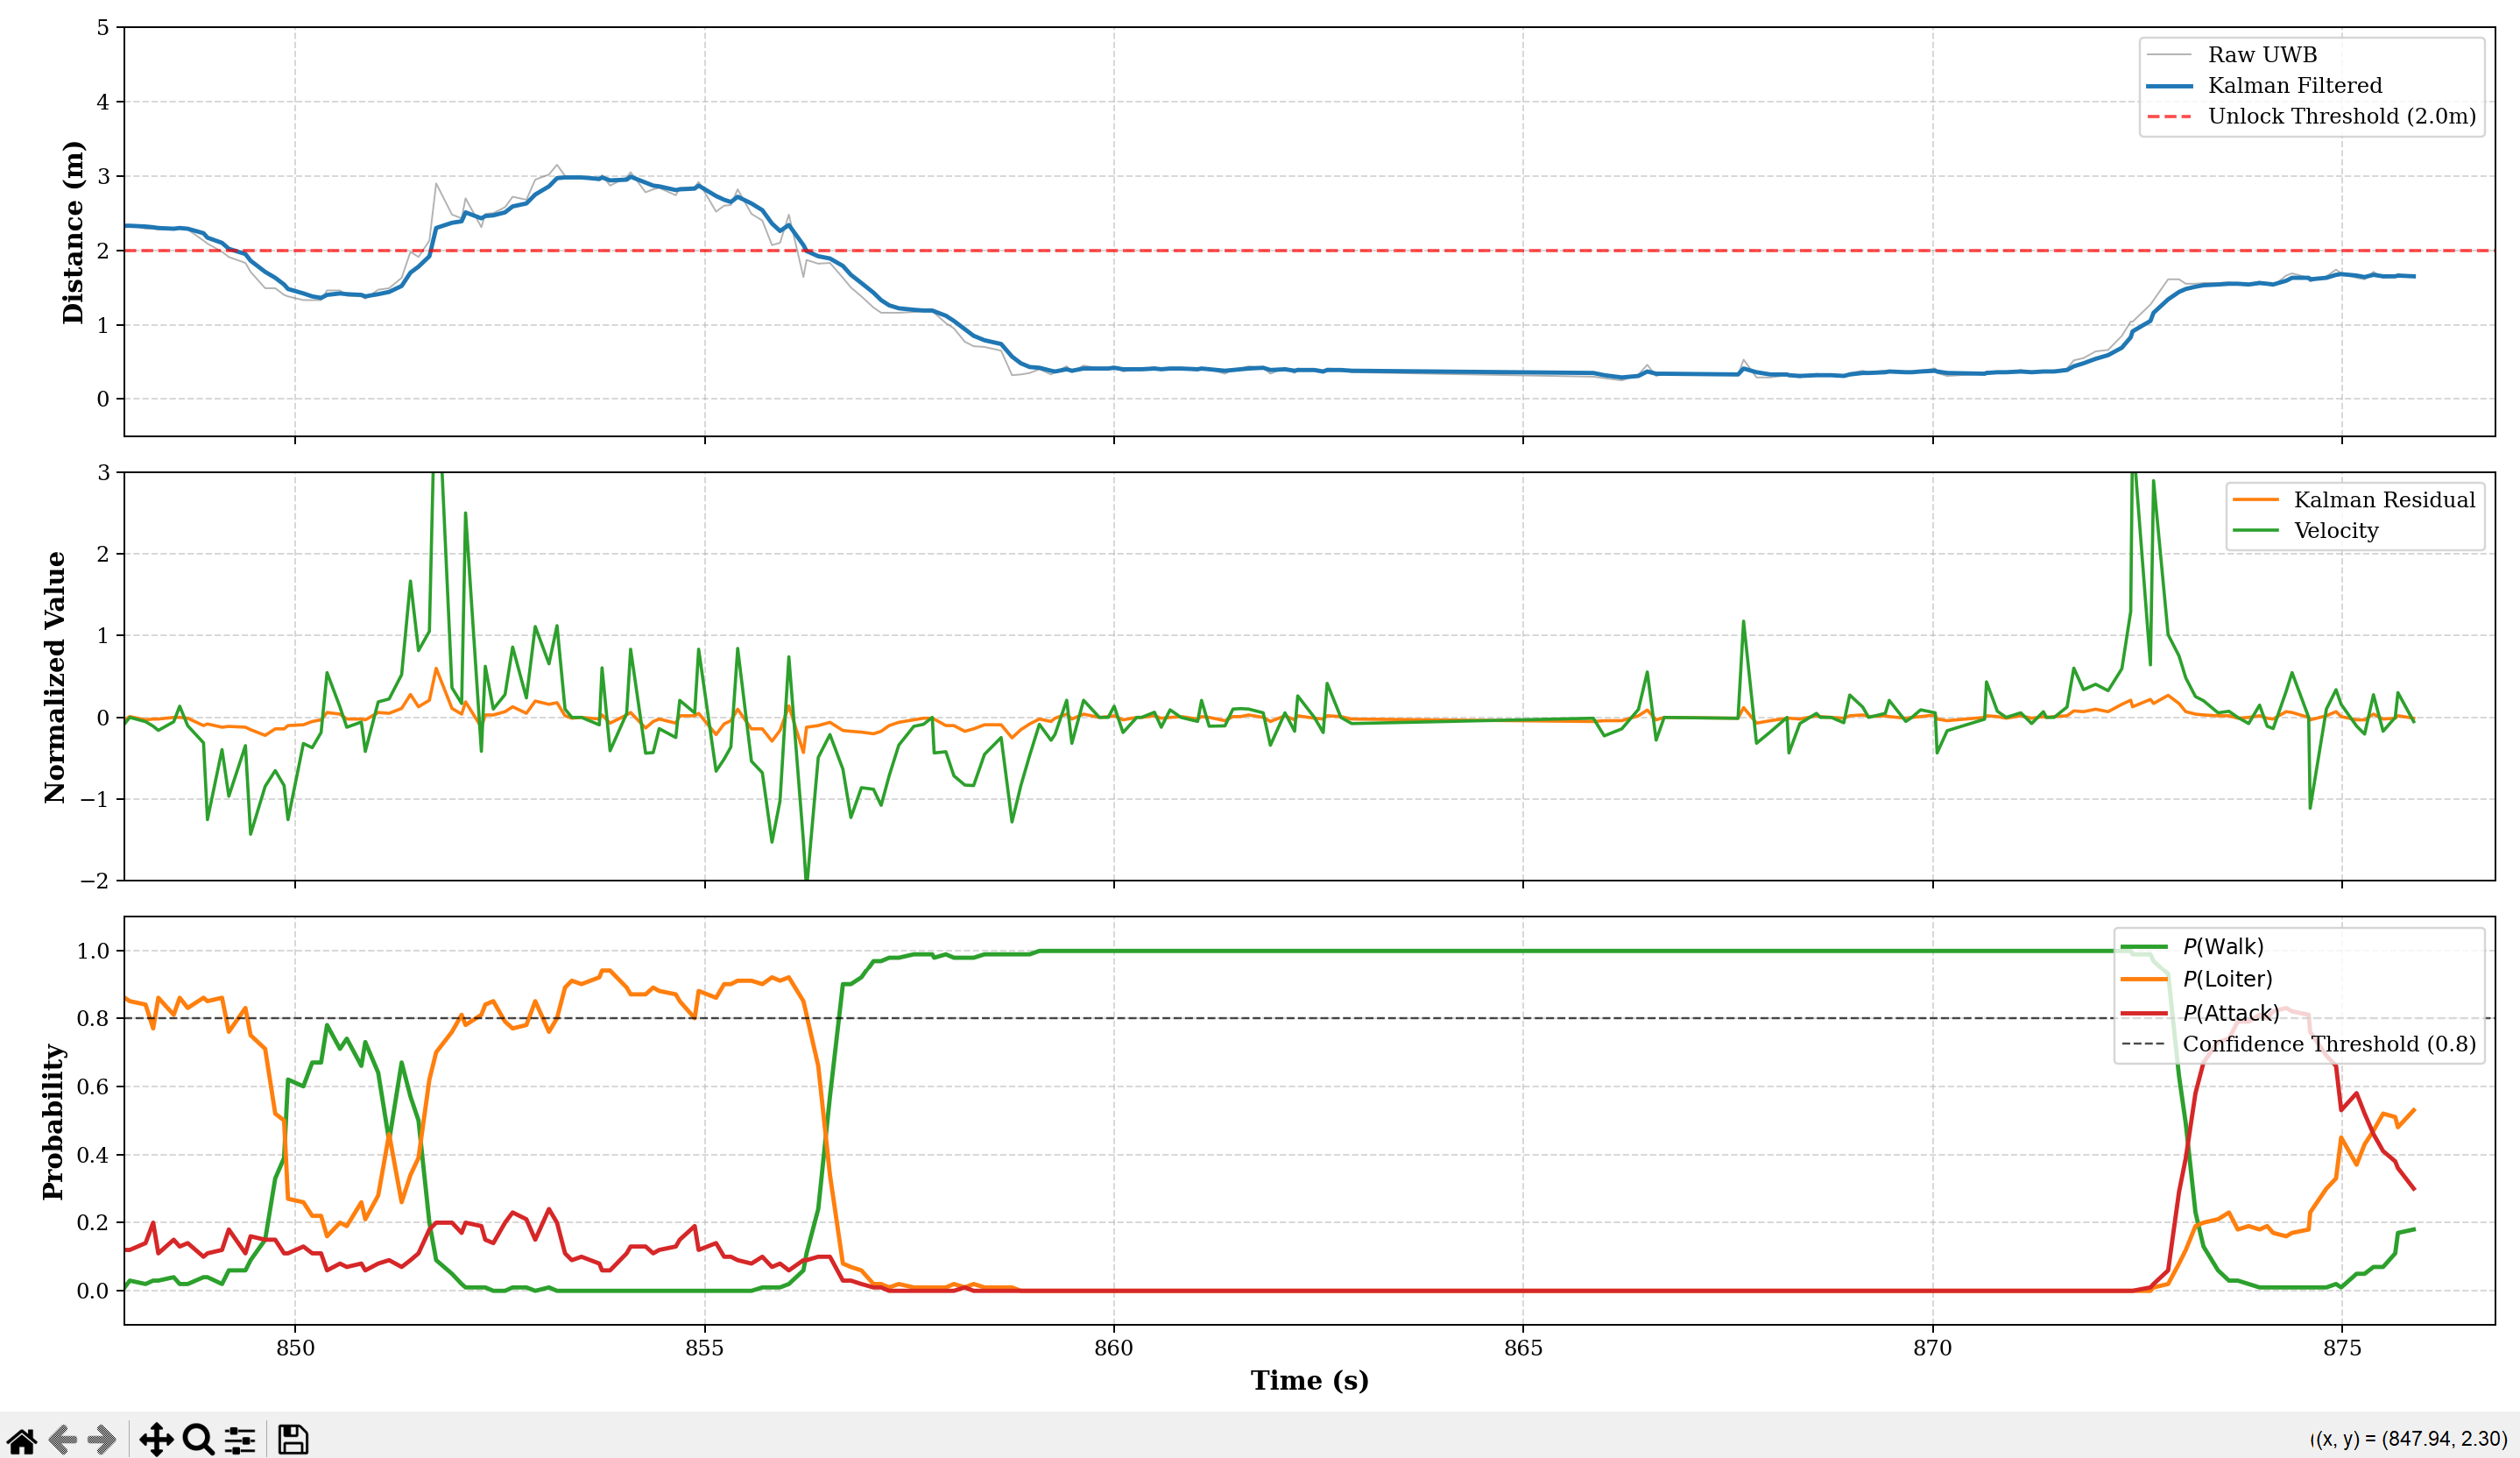
\includegraphics[width=0.8\textwidth]{image/section5/kalman_filter.png}
%     \caption{Đồ thị đối chứng dữ liệu UWB thô và dữ liệu sau bộ lọc Kalman}
%     \label{fig:ai_result}
% \end{figure}

% Sự kết hợp giữa bộ lọc Kalman và tầng nhận diện ý định TinyML (\textbf{đang hiện thực}) hướng tới nâng tầm hệ thống từ một thiết bị đo khoảng cách thuần túy thành một hệ thống nhận thức ngữ cảnh (Context-aware). Các kết quả kiểm thử trên đã chứng minh sự vận hành ổn định và tính đúng đắn của toàn bộ kiến trúc hệ thống Tri-Radio, đáp ứng toàn diện tiêu chuẩn an ninh nghiêm ngặt dành cho giải pháp truy cập phương tiện thông minh.